\documentclass{beamer}

\usepackage[ngerman]{babel}
\usepackage[utf8]{inputenc}
\usepackage{url}
\usepackage{hyperref}
\usepackage{eurosym}
\usepackage{bibgerm}
\usepackage{bibentry}
\usepackage{graphicx}
\bibliographystyle{unsrt}

\mode<presentation>{
	\definecolor{LogoRed}{RGB}{219,00,31}
	\definecolor{LogoGray}{RGB}{86,86,80}
	
	\useoutertheme[width=2.1cm]{sidebar}
	\useinnertheme{rounded}
	\setbeamercolor{normal text}{fg=black,bg=white}
	\setbeamercolor{palette sidebar primary}{use=normal text,fg=normal text.fg}
	\setbeamercolor{title}{fg=LogoRed}
	\setbeamercolor{frametitle}{fg=LogoRed}
	\setbeamercolor{structure}{fg=LogoRed}
	\setbeamercolor{section in sidebar}{fg=LogoRed}
	\setbeamercolor{subsection in sidebar}{fg=LogoRed}
	
	\usefoottemplate{\vbox{\tinycolouredline{LogoGray!25}{\hspace{4pt}\hspace{15pt}\insertdate\hfill\insertshortinstitute\hfill \insertframenumber{}/\inserttotalframenumber}}}
	
	\setbeamertemplate{section in toc}{\inserttocsectionnumber.~\inserttocsection\par}
	\setbeamertemplate{subsection in toc}{\hspace*{2em}\inserttocsectionnumber.\inserttocsubsectionnumber~\inserttocsubsection}
	\AtBeginSubsection[] {
		\begin{frame}<beamer>
			\frametitle{Outline}
			\tableofcontents[currentsection,sectionstyle=show/show,subsectionstyle=show/shaded/hide]
		\end{frame}
	}
}

\title{Man-in-the-Middle-Angriffe}
\subtitle{Praktikum Datenschutz und Datensicherheit \\ Sommersemester 2016}
\author[Fabian Uhlmann \and{Diana Irmscher}]{Fabian Uhlmann
\and {Diana Irmscher}}
\institute[Hochschule für angewandte Wissenschaften München]{Fakultät für Informatik und Mathematik
\and{Hochschule für angewandte Wissenschaften München}}
\logo{
\includegraphics[height=1.0cm]{logo_hm.png}}
\date{\today}

\setbeamertemplate{navigation symbols}{}

\begin{document}
	\maketitle
	
	\section{Begrüßung}
	
	\begin{frame} %% Die Vortragenden stellen sich vor
		\frametitle{Vorstellung}
		\begin{columns}
			\column{.47\textwidth}
			
\includegraphics[width=0.7\textwidth]{uhlmann.jpg}\\
			\textbf{Fabian Uhlmann}
			\\
			Informatik, Bachelor
			\column{.47\textwidth}
			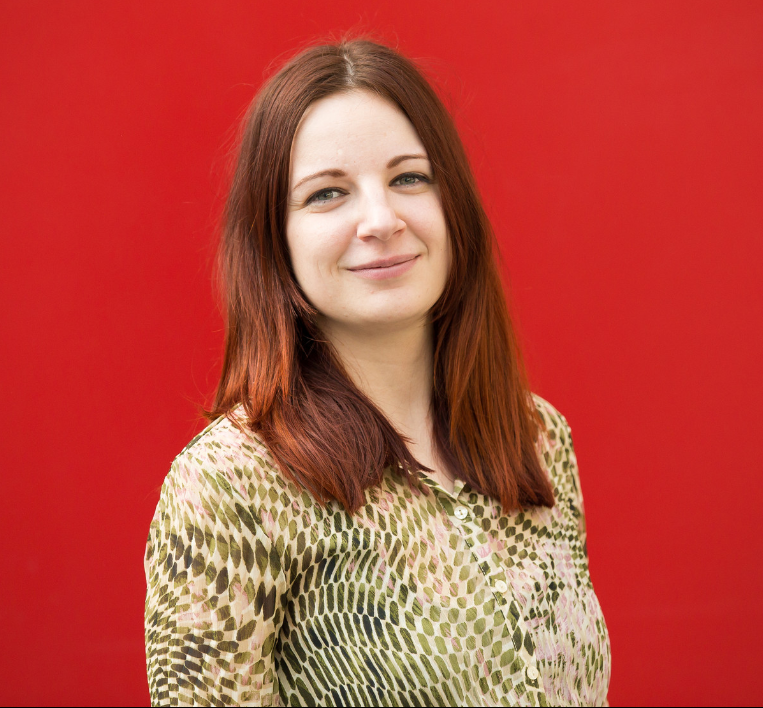
\includegraphics[width=0.725\textwidth]{irmscher.png}\\
			\textbf{Diana Irmscher}
			\\
			Informatik, Bachelor
		\end{columns}
		
		
		

	\end{frame}
	
	\begin{frame} %% Agenda zeigen, was noch ansteht
		\frametitle{Agenda}
		\tableofcontents
	\end{frame}
	
	\section{Man in the Middle im Web}
	
		\begin{frame}
			\frametitle{Aufgabenstellung}
			Dell und Lenovo haben demonstriert, dass man mit Man-in-the-Middle
			Angriffen die Sicherheit eines Systems sehr effizient aushebeln kann.
			Wie funktioniert ein derartiger Angriff und was kann man tun, um sich
			zu schützen.
	    \end{frame}
	     \subsection*{Einführung}
	     \begin{frame}
	     	\frametitle{Man in the Middle (MITM)}
	     	\begin{minipage}[t]{0.8\linewidth}
	     		%	\centering
	     		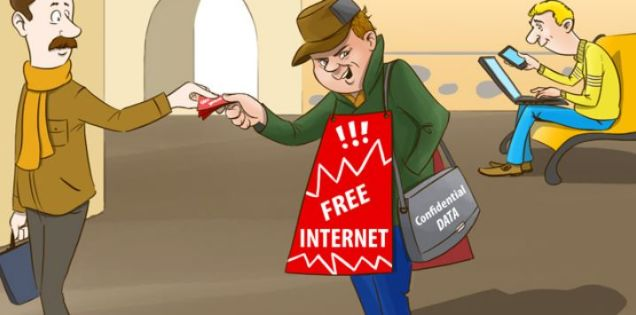
\includegraphics[width=0.8\linewidth]{images_fabian/mitm.jpg}
	     		\newline Quelle: [1]
	     	\end{minipage}% <- sonst wird hier ein Leerzeichen eingefügt
	     	\hfill
	     	\begin{minipage}[t]{0.7\linewidth}
	     	%	\centering
	     		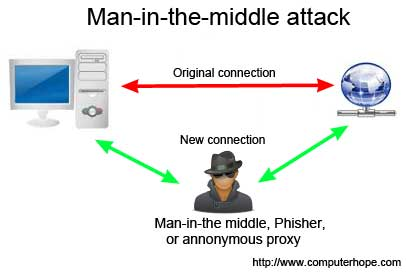
\includegraphics[width=0.8\linewidth]{images_fabian/mitm2.jpg}
	     		\newline Quelle: [2]
	     	\end{minipage}
	     \end{frame}
	     \begin{frame}
	     	\frametitle{HTTP(s) und Zertifikate}
	     	
	     \end{frame}
    
    \section{Man-in-the-Middle-Angriffe im geswitchten Netzwerk}
    	
    	\begin{frame}
    		\frametitle{Aufgabenstellung}
    		Es gibt Man-in-the-Middle-Angriffe nicht nur gegen SSL/TLS-Verbindungen, sondern auch gegen "normale" Netzwerkverbindungen. Sie werden von Angreifern eingesetzt, um in einem geswitchten Netz zu sniffen.
        \end{frame}
        \subsection*{Einführung}
        \begin{frame}
        	\frametitle{Hub}
            	
        \end{frame}
        
        \begin{frame}
          	\frametitle{Switch}
                  	
        \end{frame}
        
        \begin{frame}
        	\frametitle{Funktion Switch-Tabelle}
                       	
    	\end{frame}
    	
        \begin{frame}
        	\frametitle{Was ist ein geswitchtes Netzwerk}
                       	
    	\end{frame}
    	\subsection*{Angriffsmöglichkeiten}
        \begin{frame}
        	\frametitle{Angriffsmöglichkeiten}
        	
        	\begin{itemize}
        	\pause
        	\item MAC-Flooding
        	\pause
        	\item MAC-Spoofing
        	\pause
        	\item ARP-Spoofing
        	\end{itemize}
                       	
    	\end{frame}
    	
        \begin{frame}
        	\frametitle{MAC-Flooding}
                       	
    	\end{frame}
		\begin{frame}
        	\frametitle{MAC-Spoofing}
                       	
    	\end{frame}
    	\begin{frame}
    		\frametitle{ARP-Spoofing}
    	                       	
    	\end{frame}
    	\subsection*{Werkzeuge}
		\begin{frame}
        	\frametitle{Werkzeuge}
                       	
    	\end{frame}
    	\subsection*{Maßnahmen}
		\begin{frame}
        	\frametitle{Schutzmaßnahmen}
                       	
    	\end{frame}  
    	
    \section{Literatur}
    	\begin{frame}
    		\frametitle{Literatur}
    		\addcontentsline{toc}{section}{Literatur}
    		\begin{enumerate}
    			\item http://hackerspace.kinja.com/how-to-defend-yourself-against-mitm-or-man-in-the-middl-1461796382
    		\end{enumerate}
    	\end{frame}
\end{document}